\documentclass[12pt]{article}
\usepackage{../../includes/lecture_notes}
\usepackage{../../includes/math}

\begin{document}
\begin{center}
{\Huge\bf Final - Spring 2025}

\smallskip
{\large\it ECON 5753 — University of Arkansas}
\end{center}

\vspace{5mm}
\begin{enumerate}
  \item The following regression uses the ``College Scorecard'' which describes all U.S. colleges/universities. The outcome variable is the average annual earnings (\$) of students 10 years after they enroll. The explanatory variable is the median SAT Math score of the student body. I include both the variable itself and its square (quadratic in SAT math):
  \begin{codeblock}[{}]
OLS estimation, Dep. Var.: mean_earnings_10yr_after
Observations: 935
Standard-errors: Heteroskedasticity-robust
                       Estimate   Std. Error  t value   Pr(>|t|)
(Intercept)           108369.50     19595.24     5.53   4.15e-08 ***
sat_math_median         -337.94        68.78    -4.91   1.05e-06 ***
I(sat_math_median^2)       0.41         0.06     6.88   1.07e-11 ***
---
Signif. codes:  0 '***' 0.001 '**' 0.01 '*' 0.05 '.' 0.1 ' ' 1
  \end{codeblock}

  \begin{enumerate}[leftmargin = 2em]
    \item What is the predicted earnings for a school with an average SAT math score of 500 (round to the nearest dollar)?

    \item Say you take a school with an average SAT math score of 500. What is the predicted marginal change in $Y$ for a school with a 1 unit increase in average SAT math score?

    \item Can you reject the null that the relationship between SAT math score and average earnings is linear? Explain your reasoning.
  \end{enumerate}

  \newpage
  \item In class, we analyzed time-series data on the finishing time (in minutes) of the winner of the Boston Marathon. Below I report the coefficients from the following regression with piecewise linear trends:
  \vspace*{-\bigskipamount}
  $$
    \text{Finish Time}_t = \alpha + t \beta_1 + (t - 1950) * \one{t > 1950} * \beta_2 + (t - 1980) * \one{t > 1980} * \beta_3 + \epsilon_t
  $$

  \begin{codeblock}[{}]
OLS estimation, Dep. Var.: minutes
Observations: 96
Standard-errors: Newey-West (L=2)
                                  Estimate  Std. Error  t value   Pr(>|t|)
(Intercept)                         772.67     223.620     3.46   8.23e-04 ***
year                                 -0.32       0.115    -2.78   6.51e-03 **
I((year - 1950) * (year > 1950))     -0.26       0.163    -1.61   0.11
I((year - 1980) * (year > 1980))      0.57       0.077     7.35   6.77e-11 ***
---
Signif. codes:  0 '***' 0.001 '**' 0.01 '*' 0.05 '.' 0.1 ' ' 1
  \end{codeblock}

  \begin{enumerate}
    \item What is the expected finishing time in 2025? Show your work.

    \item Notice that $\hat{\beta}_2$ is not statistically significant. What does this suggest about the time-trends in finishing times.

    \item Looking into the future, how many minutes (or fractions of minutes) do we expect the finishing time to decrease each year?
  \end{enumerate}




  \vspace*{2\bigskipamount}
  \item Say you have a sample of stores where you observe the average daily revenue and the number of employees on the sales floor. You regress the average daily revenue on the number of employees and estimate a coefficient of $\hat{\beta}_1 = 2247$ and a standard error of $\text{SE}(\hat{\beta}_1) = 980$.
  \begin{enumerate}
    \item Interpret this coefficient estimate in words.

    \item The company does not want to increase the number of staff if these results are not statistically significant. Perform and report a test of the null that $\beta_1 = 0$. The company is risk adverse and want you to use a level of significance of $\alpha = 0.01$ (the z-score associated with this is $2.58$).
  \end{enumerate}



  \newpage
  \item You are an analyst at a large retail company.
  The retail company has a goal of "improving customer in-store experience".
  The company surveys a random sample of customer sentiment every week, asking customers to rate their in-store experience on a scale from 1 to 10.

  \begin{enumerate}
  \item Explain why simply reporting the most recent week's average score might not be the best way to measure progress.

  \item Suppose there is a sudden, genuine improvement in customer experience due to a new training intervention. Compare how quickly the 5-week moving average and the most recent week's score would reflect this change. Which would you recommend for reporting progress, and why?

  \item Suppose the company wants to test whether the new training intervention has had a statistically significant impact on customer sentiment.
        Describe a time-series regression you could run to test if there is a statistically significant jump in responses after the intervention.
        Describe the hypothesis test you would use after running this regression.
  \end{enumerate}


  \newpage
  \item On the following page, I present time-series data on the $\log$ of the daily number of airline passengers (millions).
  Additionally, I present output from \texttt{feols} from a time-series regression.
  Use both the figure and the regression output to answer the following questions:

  \begin{enumerate}
    \item Forecast the the daily number of airline passengers for the January 1st in 1965 (note the outcome in the regression is logged, so you need to exponentiate). Show your work. What are you assuming when forecasting multiple years into the future?

    \item Interpret the coefficient on the \texttt{July} indicator. Form a 95\% confidence interval for this coefficient and comment on its statistical significance.

    \item Describe how you might change this regression model to test if the number of passengers in June is statistically significantly larger than May.

    \item You might be concerned that your time-series model is missing some predictable patterns. Describe in words what you could do to visually assess that.
  \end{enumerate}
\end{enumerate}

\newpage
\begin{figure}[h!]
  \caption{$\log$ Daily number of passengers (millions)}
  \label{fig:bitcoin}

  \vspace*{-2\bigskipamount}
  \begin{center}
  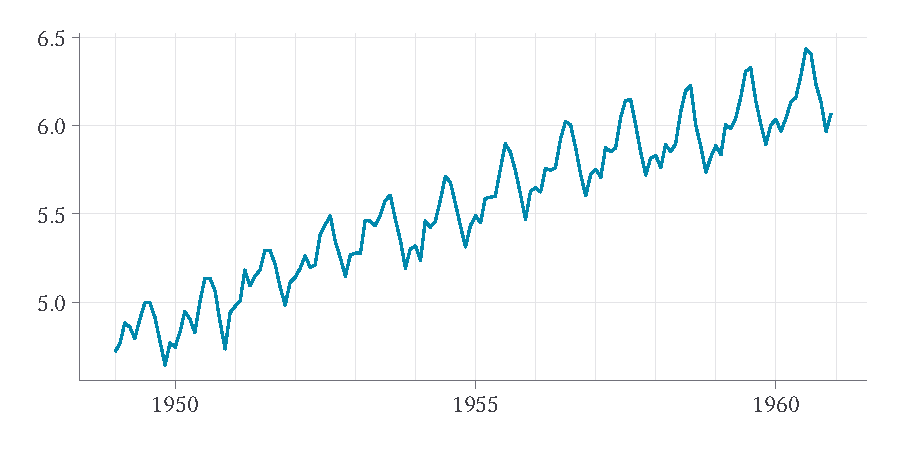
\includegraphics[width = 0.8\textwidth]{figures/log_n_passengers_airline.pdf}
  \end{center}
\end{figure}

\vspace*{-\bigskipamount}
\begin{codeblock}[{}]
OLS estimation, Dep. Var.: log(n_passengers)
Observations: 144
Standard-errors: Newey-West (L=2)
                  Estimate  Std. Error   t value   Pr(>|t|)
(Intercept)        -230.75       4.690    -49.20  < 2.2e-16 ***
year                  0.12       0.002     50.36  < 2.2e-16 ***
month::February      -0.01       0.020     -0.60   5.43e-01
month::March          0.13       0.023      5.46   1.99e-07 ***
month::April          0.10       0.023      4.59   9.53e-06 ***
month::May            0.11       0.024      4.70   5.91e-06 ***
month::June           0.25       0.024     10.43  < 2.2e-16 ***
month::July           0.36       0.023     15.76  < 2.2e-16 ***
month::August         0.36       0.023     16.20  < 2.2e-16 ***
month::September      0.23       0.020     11.15  < 2.2e-16 ***
month::October        0.10       0.020      4.92   2.31e-06 ***
month::November      -0.03       0.020     -1.76   7.93e-02 .
month::December       0.09       0.016      5.69   6.73e-08 ***
---
Signif. codes:  0 '***' 0.001 '**' 0.01 '*' 0.05 '.' 0.1 ' ' 1
\end{codeblock}


\end{document}
